\chapter*{List of Appendices}
\addcontentsline{toc}{chapter}{Appendix}

\begin{itemize}[label={}]
\item Appendix 1: \hypertarget{pUA66seq}{\href{https://drive.google.com/open?id=1oHOr45i53oj1ZvaJO2rwhhKW336-1qDa}{Sequence of pUA66 vector}}
\item Appendix 2: \hypertarget{p139seq}{\href{https://drive.google.com/open?id=1eTZO0u8nTtbIphnsHlNvB4G_L2-LnJ-f}{Sequence of pU139 vector}}
\item Appendix 3: \hypertarget{placZalign}{\href{https://drive.google.com/open?id=1uxseqbHVccpsxmKUuVl5_nBY2wEvpF8J}{\tax{placZ} promoter sequence alignment with vectors and references}}
\item Appendix 4: \hypertarget{precAalign}{\href{https://drive.google.com/open?id=1g5AUZ4vEhNVGWuKy9A7augQ2beI5EW9o}{\tax{precA} promoter sequence alignment with vector and reference}}
\item Appendix 5: \hypertarget{pLW001}{\href{https://drive.google.com/open?id=1HhTVjaBZxkOQPb05qaPJYQk1XmyXM7zO}{pLW001 plasmid sequence}}
\item Appendix 6: \hypertarget{pADOUCHseq}{\href{https://drive.google.com/open?id=1RT7LigW9waKPSw4mTKGJVCJavP3P0kWW}{Sequence alignment of 1:3(1) and 1:5(1) clones with expected reference}}
\item Appendix 7: \hypertarget{pADOUCHwhole}{\href{https://drive.google.com/open?id=1kS7Ih-cgBlwvxuMc4spGqSF4MdvcVV9f}{Sequence of constructed pADOUCH vector}}
\end{itemize}



\begin{figure}[h!!!]
  \centering
  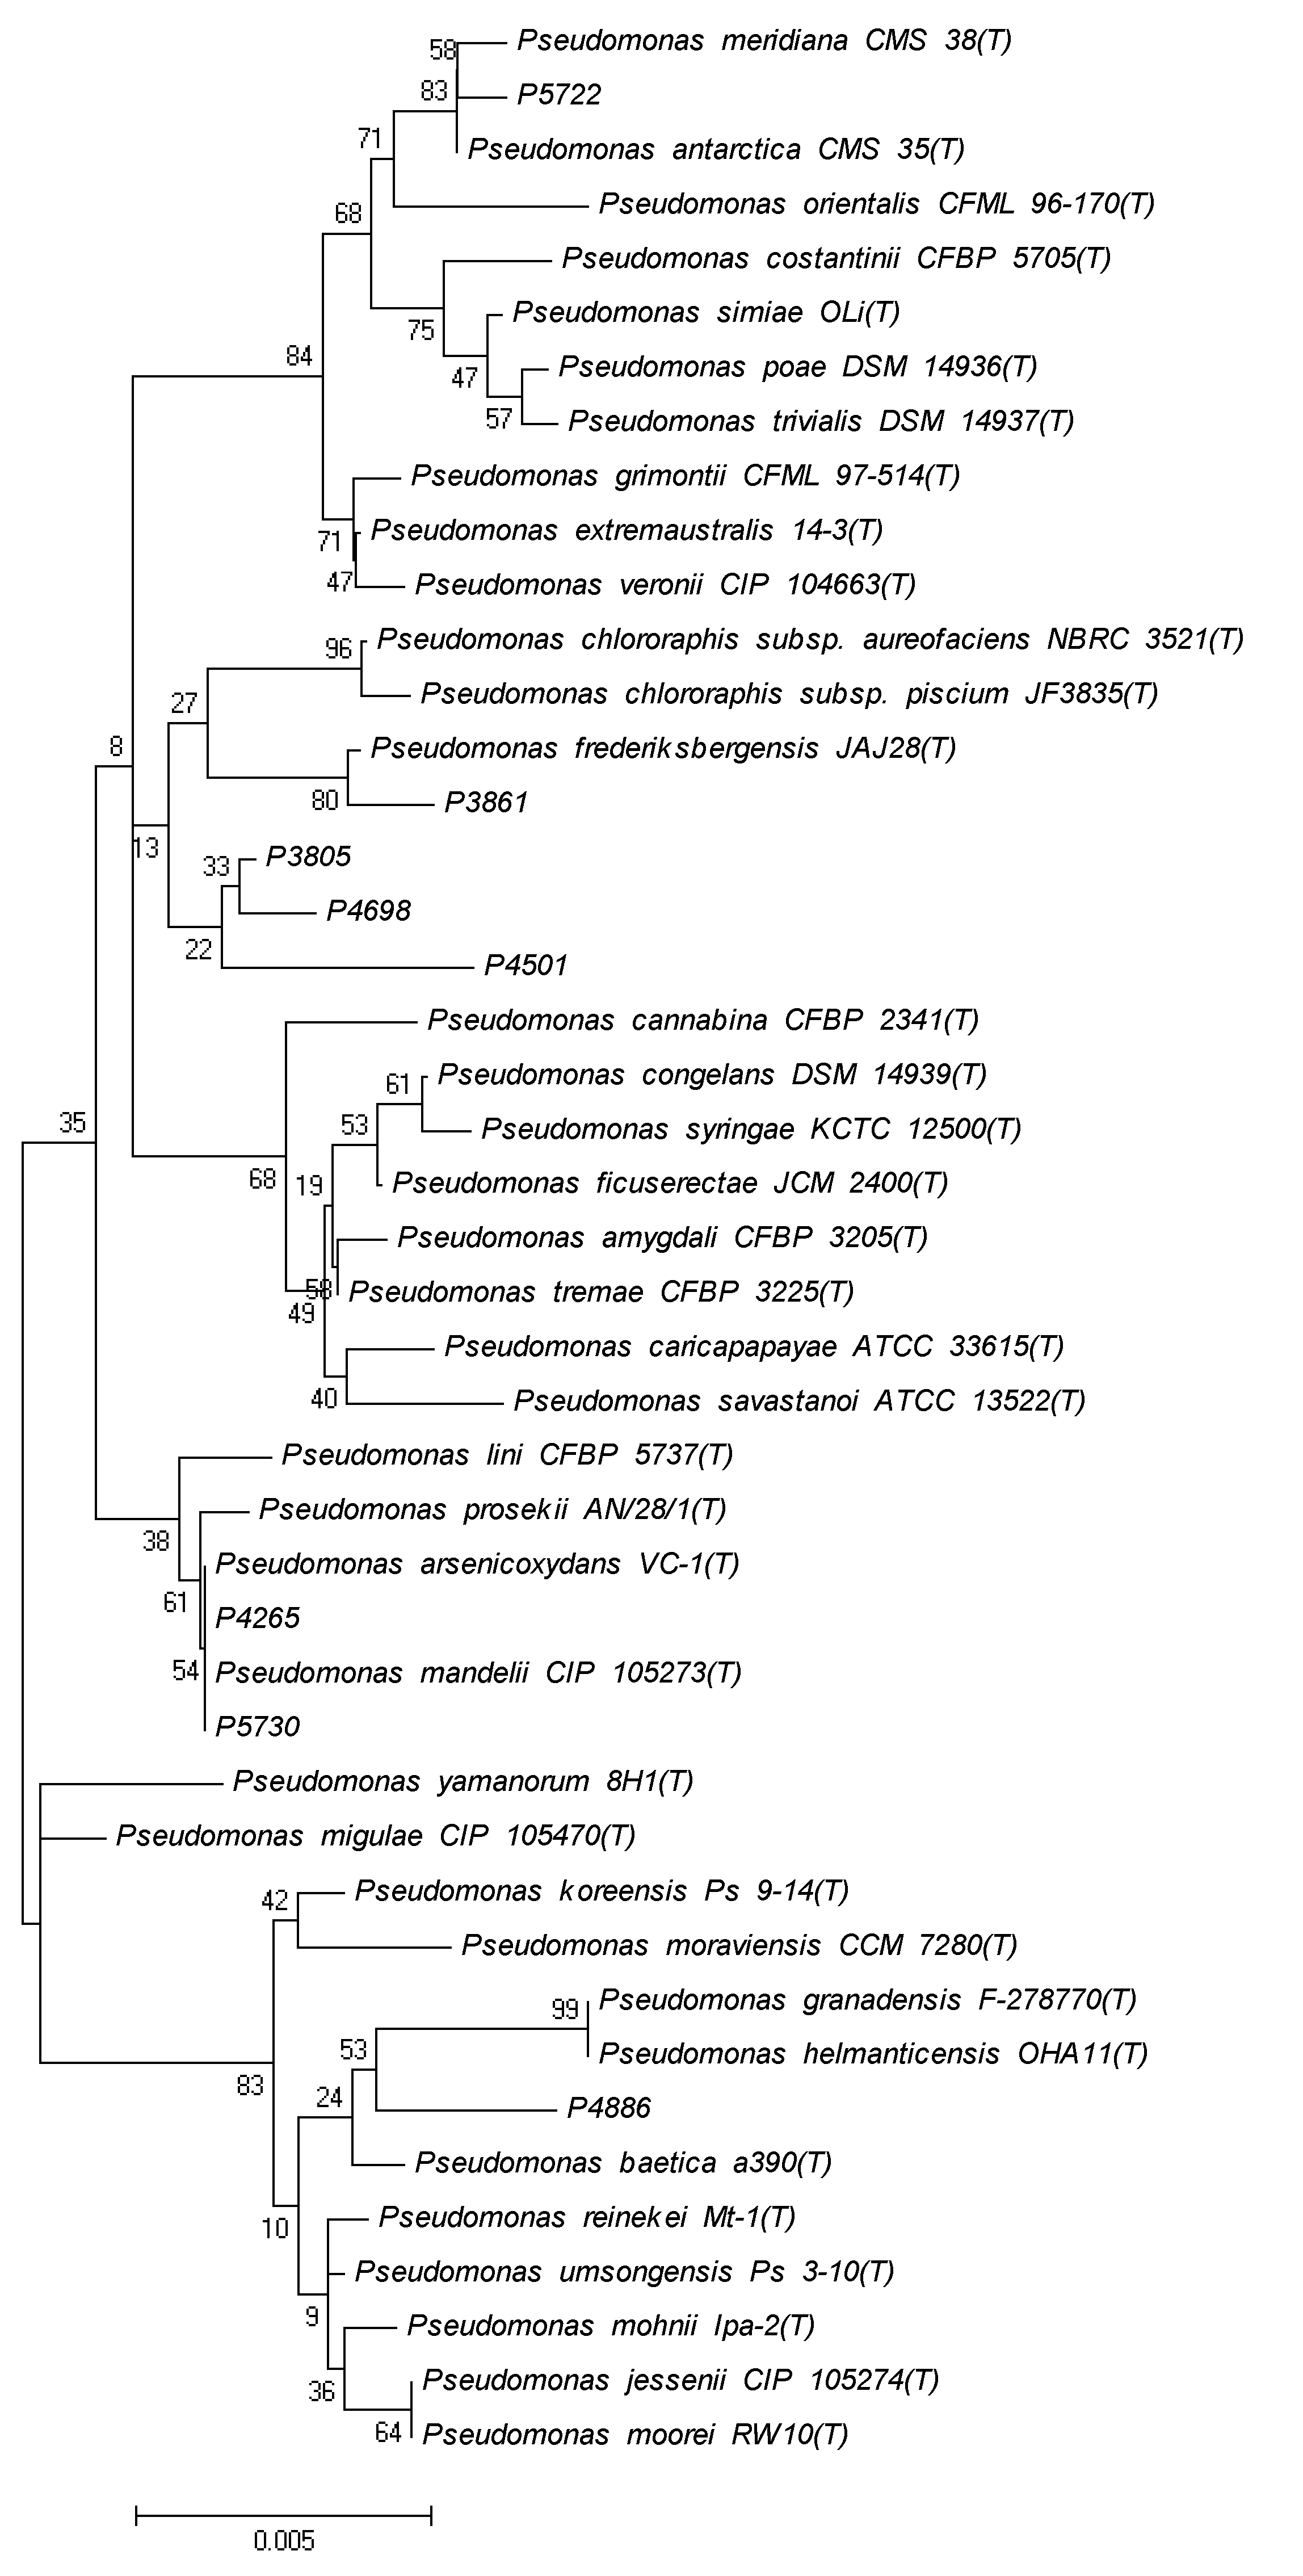
\includegraphics[scale=0.50]{text/Pictures/160508_16S_ML_clustalW_Bootstrap-consensus.png}
	\caption{Fylogenetický strom na základě analýzy genu \tax{rrs} dle metody Maximum-likelihood}
	\label{rrs_ML}
\end{figure}
\pagebreak

\begin{figure}[h!!!]
  \centering
  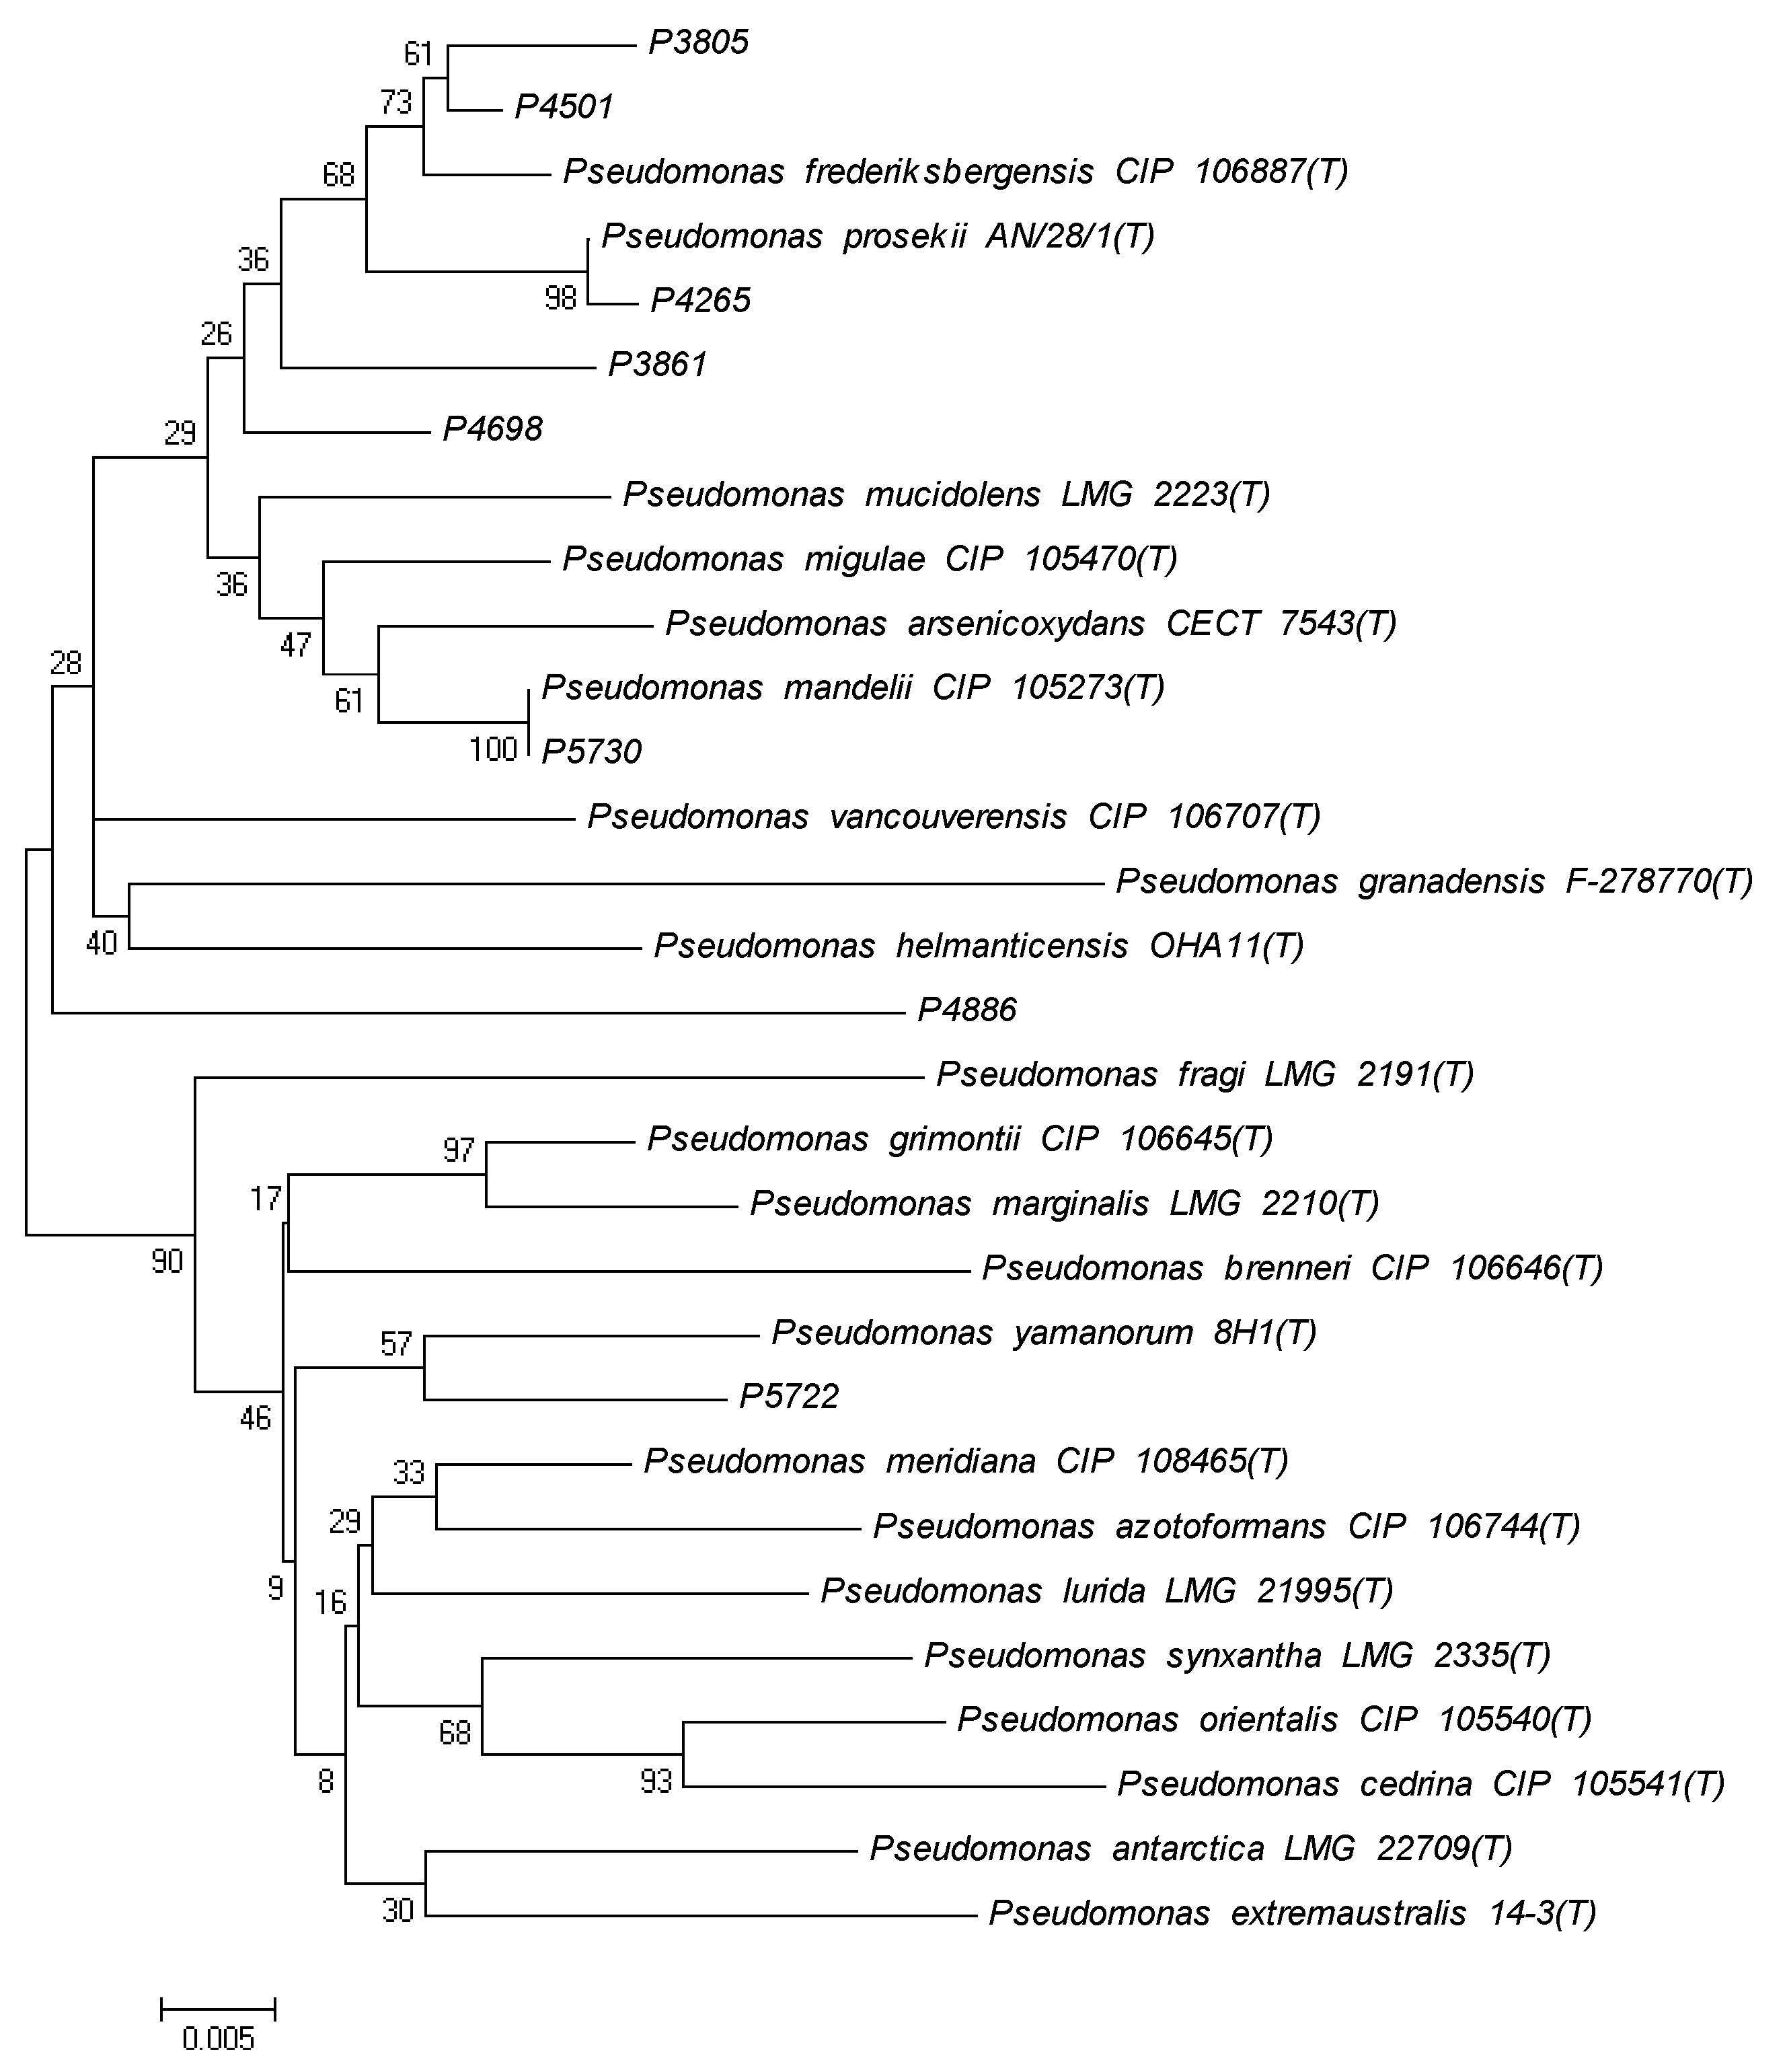
\includegraphics[scale=0.50]{text/Pictures/160508_rpoB_multifasta_doplnek_ML_clustalW_Bootstrap-consensus.png}
	\caption{Fylogenetický strom na základě analýzy genu \tax{rpoB} dle metody Maximum-likelihood}
	\label{rpoB_ML}
\end{figure}
\pagebreak

\begin{figure}[h!!!]
  \centering
  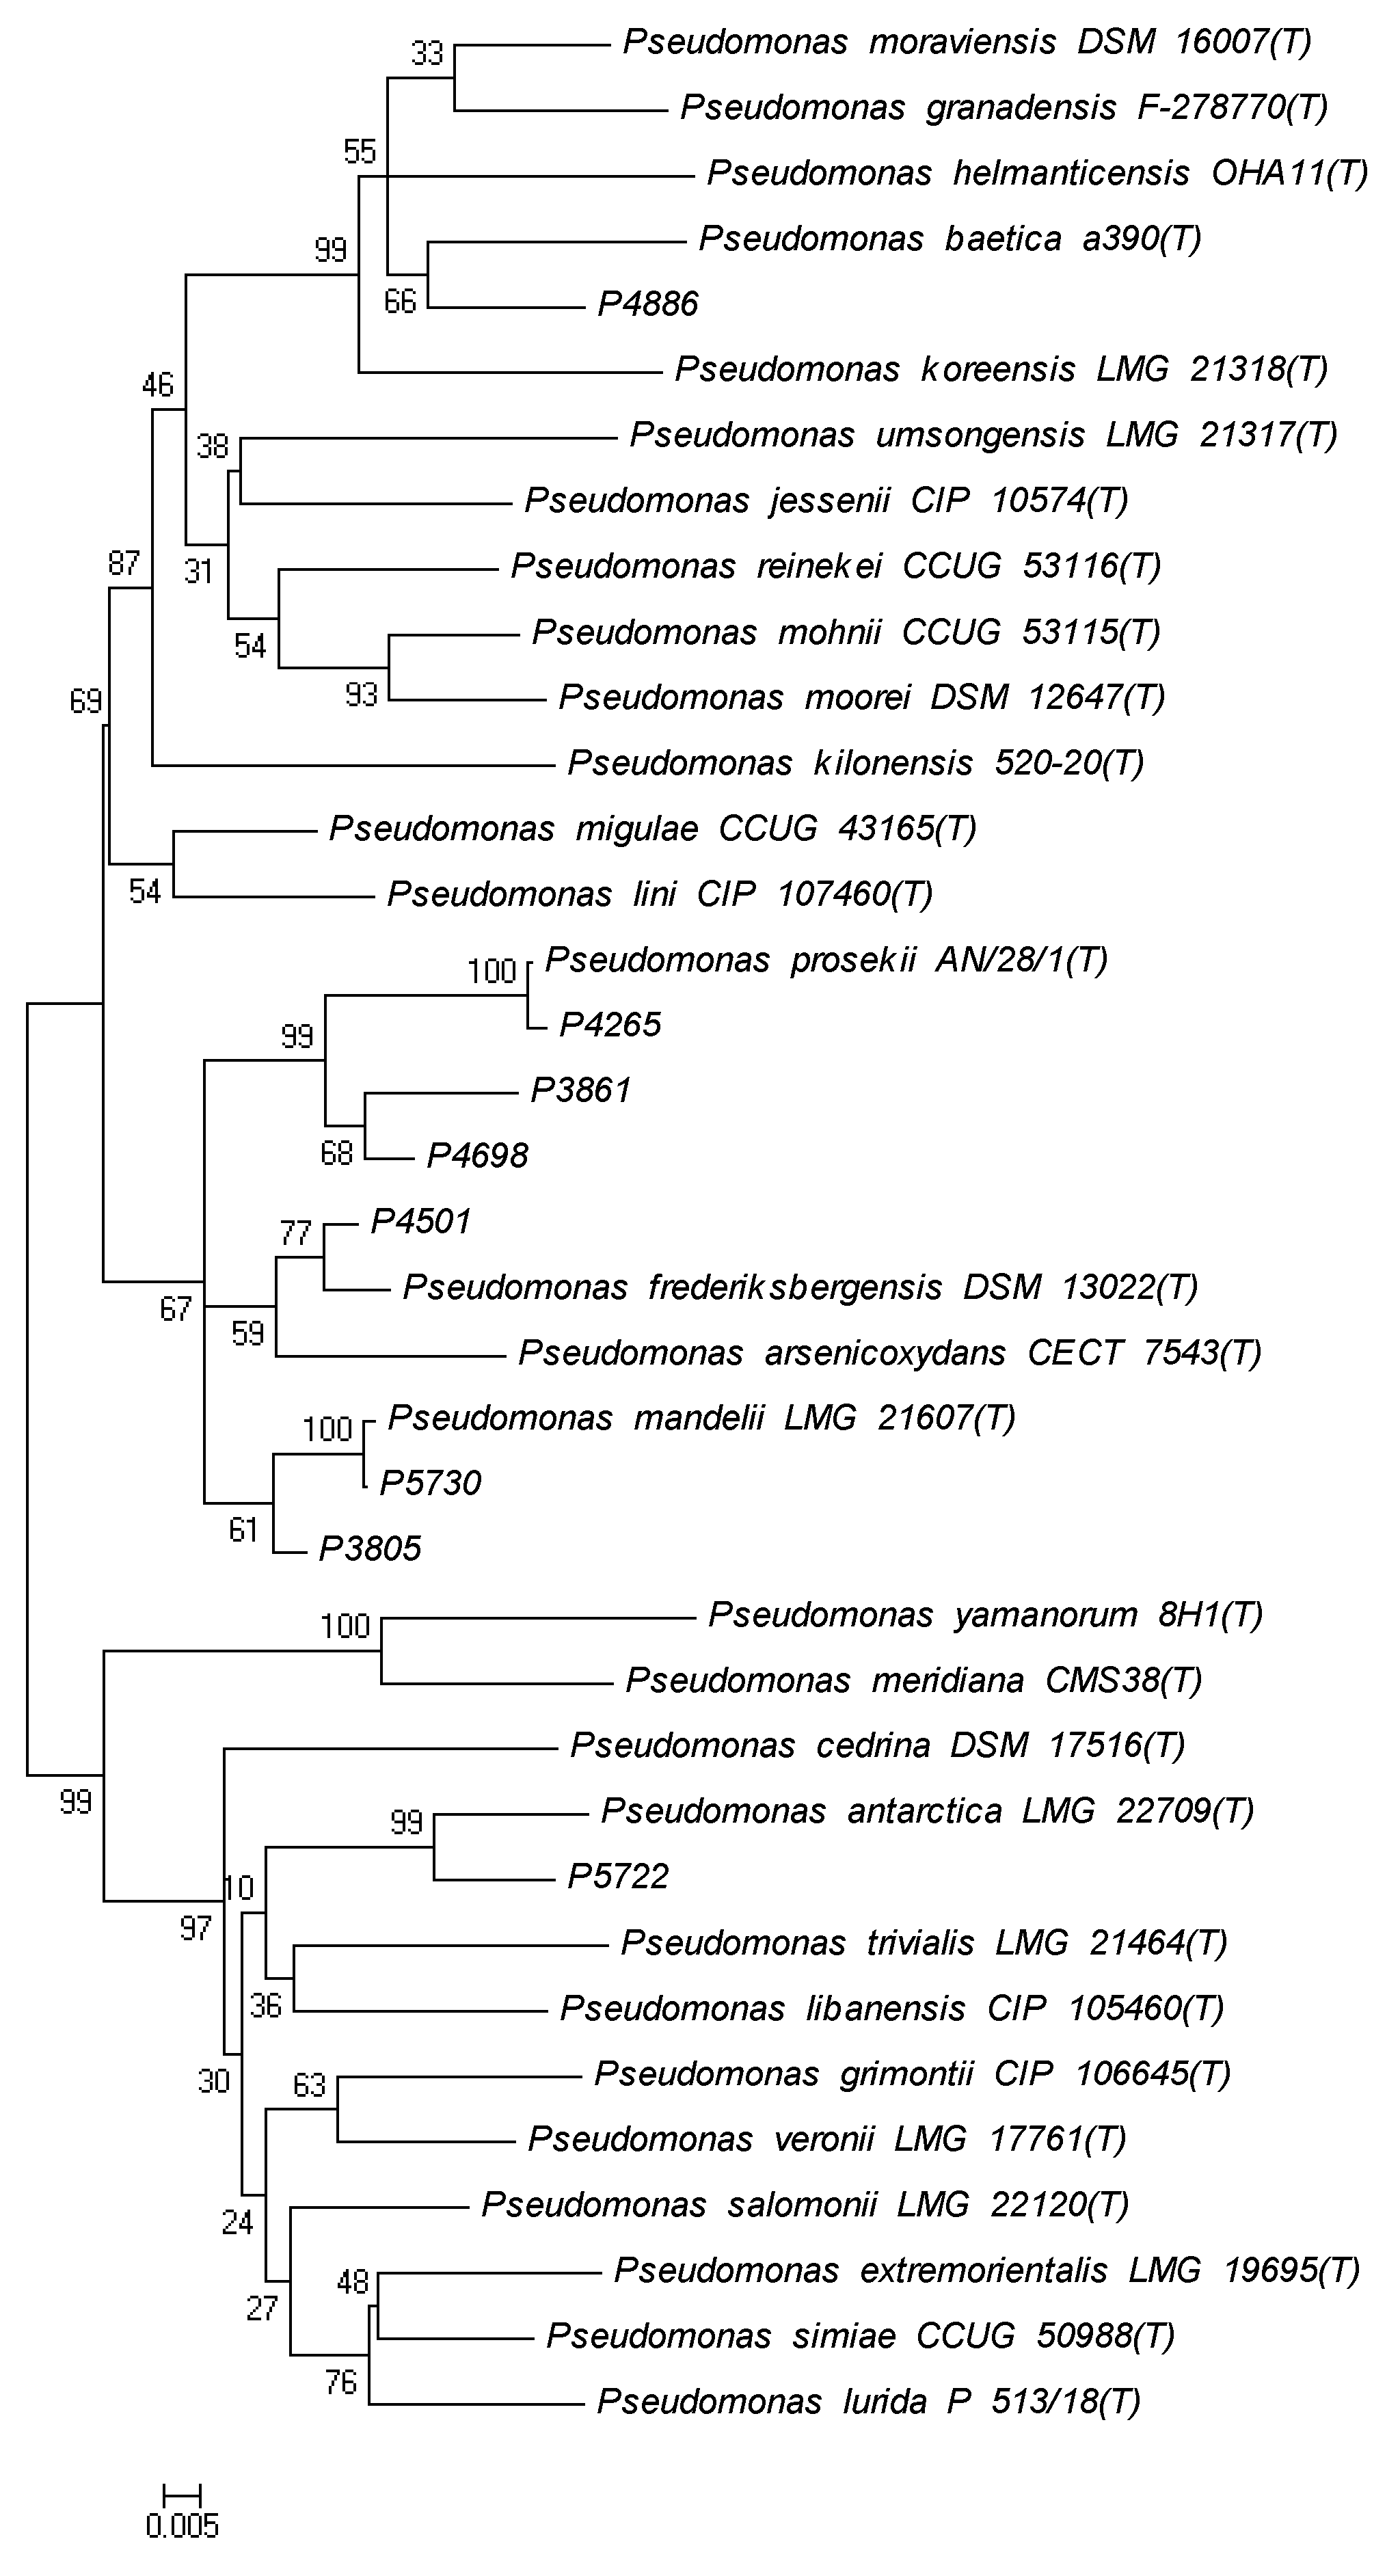
\includegraphics[scale=0.50]{text/Pictures/160508_rpoD_multifasta_doplnek_ML_clustalW_Bootstrap-consensus.png}
	\caption{Fylogenetický strom na základě analýzy genu \tax{rpoD} dle metody Maximum-likelihood}
	\label{rpoD_ML}
\end{figure}
\clearpage

%\includepdf[link, linkname=SPARC, pages=1, landscape, fitpaper]{text/Pictures/Sbornik-SPARC2016.pdf}

%\includepdf[link, linkname=SPARC, pages=55, landscape, fitpaper]{text/Pictures/Sbornik-SPARC2016.pdf}

%Here is a \hyperlink{anal_vse_ward_jacc_color3.pdf.19}{hyperlink to page 19} of anal_vse_ward_jacc_color3.pdf.

%\medskip

%%%%%%%%%%%%%%%%%%%%%%%%%%%%%%%%%%%%
%%%%%%%%% GENERUJ TEXT %%%%%%%%%%%%%
%%%%%%%%%%%%%%%%%%%%%%%%%%%%%%%%%%%%

\cleardoublepage
